\documentclass[a4paper,14pt]{extarticle}

\usepackage[utf8x]{inputenc}
\usepackage[T1,T2A]{fontenc}
\usepackage[russian]{babel}
\usepackage{hyperref}
\usepackage{indentfirst}
\usepackage{here}
\usepackage{array}
\usepackage{graphicx}
\usepackage{caption}
\usepackage{subcaption}
\usepackage{chngcntr}
\usepackage{amsmath}
\usepackage{amssymb}
\usepackage{pgfplots}
\usepackage{pgfplotstable}
\usepackage[left=2cm,right=2cm,top=2cm,bottom=2cm,bindingoffset=0cm]{geometry}
\usepackage{multicol}
\usepackage{askmaps}
\usepackage{titlesec}
\usepackage{listings}
\usepackage{color}
\usepackage{courier}

\definecolor{green}{rgb}{0,0.6,0}
\definecolor{gray}{rgb}{0.5,0.5,0.5}
\definecolor{purple}{rgb}{0.58,0,0.82}

\lstset{
	language=Verilog,
	backgroundcolor=\color{white},   
	basicstyle=\small\ttfamily,
	commentstyle=\color{green},
	keywordstyle=\color{blue},	
	numberstyle=\tiny\color{gray},
	stringstyle=\color{purple},
	breakatwhitespace=false,
	breaklines=true,
	captionpos=b,
	keepspaces=true,
	numbers=left,
	numbersep=5pt,
	showspaces=false,
	showstringspaces=false,
	showtabs=false,
	tabsize=4,
	frame=single,
	inputpath={../quartus/},
	literate={~} {$\sim$}{1}
}

\renewcommand{\le}{\ensuremath{\leqslant}}
\renewcommand{\leq}{\ensuremath{\leqslant}}
\renewcommand{\ge}{\ensuremath{\geqslant}}
\renewcommand{\geq}{\ensuremath{\geqslant}}
\renewcommand{\epsilon}{\ensuremath{\varepsilon}}
\renewcommand{\phi}{\ensuremath{\varphi}}
\renewcommand{\thefigure}{\arabic{figure}} 	
\renewcommand*\not[1]{\overline{#1}}

\titleformat*{\section}{\large\bfseries} 
\titleformat*{\subsection}{\normalsize\bfseries} 
\titleformat*{\subsubsection}{\normalsize\bfseries} 
\titleformat*{\paragraph}{\normalsize\bfseries} 
\titleformat*{\subparagraph}{\normalsize\bfseries} 

\counterwithin{figure}{section}
\counterwithin{equation}{section}
\counterwithin{table}{section}
\newcommand{\sign}[1][5cm]{\makebox[#1]{\hrulefill}}
\graphicspath{{../pics/}}
\captionsetup{justification=centering,margin=1cm}
\def\arraystretch{1.3}
\setlength\parindent{5ex}
\titlelabel{\thetitle.\quad}

\begin{document}

\begin{titlepage}
\begin{center}
	Санкт-Петербургский Политехнический Университет Петра Великого\\[0.3cm]
	Институт компьютерных наук и технологий \\[0.3cm]
	Кафедра компьютерных систем и программных технологий\\[4cm]
	
	\textbf{ОТЧЕТ}\\ 
	\textbf{по лабораторной работе}\\[0.5cm]
	\textbf{SystemVerilog №4}\\[0.1cm]
	Автоматизация проектирования\\ дискретных устройств\\[4.0cm]
\end{center}

\begin{flushright}
	\begin{minipage}{0.45\textwidth}
		\textbf{Работу выполнил студент}\\[3mm]
		группа 33501/4 \hspace*{9mm} Дьячков В.В.\\[5mm]
		\textbf{Преподаватель}\\[5mm]
		\sign[1.5cm] \hspace*{1mm} к.т.н., доц. Филиппов А.С. \\[5mm]
	\end{minipage}
\end{flushright}

\vfill

\begin{center}
	Санкт-Петербург\\
	\the\year
\end{center}
\end{titlepage}

\addtocounter{page}{1}
\counterwithin{lstlisting}{section}

\tableofcontents
\lstlistoflistings
\listoffigures
\newpage

\section{Задание}

\begin{itemize}
	\item Для задания \code{lab4_2} осеннего семестра для каждого модуля (счетчик-делитель, регистр с обратными связями) и для описания верхнего уровня, на языке Verilog создать описание тестов:
		\begin{itemize}
			\item Тест класса 1:
				\begin{itemize}
					\item Для счетчика-делителя -- \code{tb1_labs_11cd.v};
					\item Для регистра -- \code{tb1_labs_11r.v};
					\item Для описания верхнего уровня -- \code{tb1_ labs_11top.v}.
				\end{itemize}
			\item Тест класса 2 с вычислением результата:
				\begin{itemize}
					\item Для счетчика-делителя -- \code{tb2_labs_11cd.v};
					\item Для регистра -- \code{tb2_labs_11r.v};
					\item Для описания верхнего уровня -- \code{tb2_ labs_11top.v}.
				\end{itemize}
			\item Тест класса 2 с чтением файлов
				\begin{itemize}
					\item Для счетчика-делителя -- \code{tb2_labs_11cd.v} (файл с тестовыми воздействиями -- \code{input_labs_11cd.dat}, файл с ожидаемыми результатами -- \code{exp_labs_11cd.dat});
					\item Для регистра -- \code{tb2_labs_11r.v} (файл с тестовыми воздействиями -- \code{input_labs_11r.dat}, файл с ожидаемыми результатами -- \code{exp_labs_11r.dat});
					\item Для описания верхнего уровня -- \code{tb2_ labs_11top.v} (файл с тестовыми воздействиями -- \code{input_labs_11top.dat}, файл с ожидаемыми результатами -- \code{exp_labs_11top.dat}).
				\end{itemize}
		\end{itemize}

	\item Осуществить проверку модуля с использованием всех тестов; проверку тестов класса 2 на обработку ошибок.
\end{itemize}

\section{Описание устройства}

В листингах \ref{code:cd}--\ref{code:labs_11} приведено описание тестируемого устройства, включающего счетчик-делитель, обеспечивающий счет по модулю \code{25 000 000} и формирующий синхронный сигнал переноса, и регистр сдвига с линейной обратной связью.
\lstinputlisting[caption=\code{cd.v}, label=code:cd]{cd.v}
\lstinputlisting[caption=\code{r.v}, label=code:r]{r.v}
\lstinputlisting[caption=\code{lab4_2.v}, label=code:labs_11]{lab4_2.v}

\section{Описание тестов}
\label{sec:tests}

\subsection{Тест первого класса}

В листингах \ref{code:test1cd}--\ref{code:test1top} приведено описание тестов первого класса для каждого модуля и описания верхнего уровня.
\lstinputlisting[caption=\code{tb1_labs_11cd.v}, label=code:test1cd]{tb1_labs_11cd.v}
\lstinputlisting[caption=\code{tb1_labs_11r.v}, label=code:test1cb]{tb1_labs_11r.v}
\newpage
\lstinputlisting[caption=\code{tb1_labs_11top.v}, label=code:test1top]{tb1_labs_11top.v}

На рис. \ref{fig:test1_results} изображены временные диаграммы тестов для каждого модуля и описания верхнего уровня.
\vspace{-0.3cm}
\begin{figure}[H]
	\begin{subfigure}{\textwidth}
		\centering
		
\includegraphics[width=0.77\textwidth]{test1cd_results}
		\vspace{0.1cm}
	\end{subfigure}
	\begin{subfigure}{\textwidth}
		\centering
		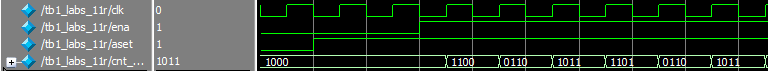
\includegraphics[width=0.99\textwidth]{test1r_results}
		\vspace{0.1cm}
	\end{subfigure}
	\begin{subfigure}{\textwidth}
		\centering
		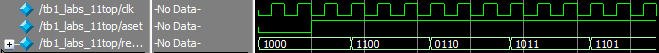
\includegraphics[width=0.9\textwidth]{test1top_results}
	\end{subfigure}
	\caption{Результаты тестов первого класса}
	\label{fig:test1_results}
\end{figure}

\subsection{Тест второго класса с вычислением результата}

В листингах \ref{code:test2cd}--\ref{code:test2top} приведено описание тестов второго класса с вычислением результата для каждого модуля и описания верхнего уровня.
\lstinputlisting[caption=\code{tb2_labs_11cd.v}, label=code:test2cd]{tb2_labs_11cd.v}
\lstinputlisting[caption=\code{tb2_labs_11r.v}, label=code:test2cb]{tb2_labs_11r.v}
\lstinputlisting[caption=\code{tb2_labs_11top.v}, label=code:test2top]{tb2_labs_11top.v}

На рис. \ref{fig:test2_results} изображена временная диаграмма теста.
\begin{figure}[H]
	\begin{subfigure}{\textwidth}
		\centering
		
\includegraphics[width=0.7\textwidth]{test2cd_results}
		\vspace{0.1cm}
	\end{subfigure}
	\begin{subfigure}{\textwidth}
		\centering
		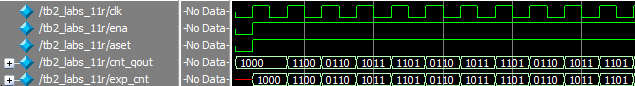
\includegraphics[width=0.87\textwidth]{test2r_results}
		\vspace{0.1cm}
	\end{subfigure}
	\begin{subfigure}{\textwidth}
		\centering
		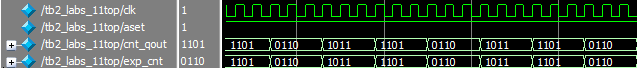
\includegraphics[width=0.88\textwidth]{test2top_results}
	\end{subfigure}
	\caption{Результаты тестов второго класса с вычислением результата}
	\label{fig:test2_results}
\end{figure}

В листинге \ref{code:test2_error} приведен вывод результатов теста верхнего уровня в консоль при внесении ошибки в вычисление ожидаемого значения.	
\begin{lstlisting}[caption=Результаты ошибочного теста второго класса с вычислением результата, label=code:test2_error, style=console]
run -all
# Expected  4, got 12
# Expected 10, got  6
# Expected 13, got 11
# Expected 14, got 13
# Expected  7, got  6
...
# Expected 10, got 13
# Expected 13, got  6
# Expected 14, got 11
# Expected  7, got 13
# Expected  3, got  6
#    Time: 1 us  Iteration: 0  Instance: /tb2_labs_11top
\end{lstlisting}

\subsection{Тест второго класса с чтением файлов}

В листинге \ref{code:test3cd}--\ref{code:test3top} приведено описание теста второго класса с чтением файлов. В данном тесте на вход модулей из файлов \code{input_labs_11cd.dat}--\code{input_labs_11top.dat}, фрагменты которых приведены в листингах \ref{code:inputcd}--\ref{code:inputtop}, подаются всевозможные значения, а ожидаемые считываются из файлов \code{exp_labs_11cd.dat}--\code{exp_labs_11top.dat}, фрагменты которых приведены в листингах \ref{code:expcd}--\ref{code:exptop}.
\lstinputlisting[caption=\code{tb2f_labs_11cd.v}, label=code:test3cd]{tb2f_labs_11cd.v}
\lstinputlisting[caption=\code{tb2f_labs_11r.v}, label=code:test3cb]{tb2f_labs_11r.v}
\lstinputlisting[caption=\code{tb2f_labs_11top.v}, label=code:test3top]{tb2f_labs_11top.v}
\begin{multicols}{2}
	\lstinputlisting[caption=\code{inp_labs_11cd.dat}, linerange={1-5, 20-24}, label=code:inputcd, style=dat]{input_labs_11cd.dat}	
	\lstinputlisting[caption=\code{inp_labs_11r.dat}, linerange={1-6}, label=code:inputcb, style=dat]{input_labs_11r.dat}	
	
	\lstinputlisting[caption=\code{exp_labs_11cd.dat}, linerange={1-5, 20-24}, label=code:expcd, style=dat]{exp_labs_11cd.dat}
	\lstinputlisting[caption=\code{exp_labs_11r.dat}, linerange={1-6}, label=code:expcb, style=dat]{exp_labs_11r.dat}
\end{multicols}
\begin{multicols}{2}
	\lstinputlisting[caption=\code{inp_labs_11top.dat}, linerange={1-9}, label=code:inputtop, style=dat]{input_labs_11top.dat}	
	
	\lstinputlisting[caption=\code{exp_labs_11top.dat}, linerange={1-9}, label=code:exptop, style=dat]{exp_labs_11top.dat}
\end{multicols}

На рис. \ref{fig:test3_results} изображена временные диаграммы тестов.
\begin{figure}[H]
	\begin{subfigure}{\textwidth}
		\centering
		
\includegraphics[width=0.81\textwidth]{test3cd_results}
		\vspace{0.1cm}
	\end{subfigure}
	\begin{subfigure}{\textwidth}
		\centering
		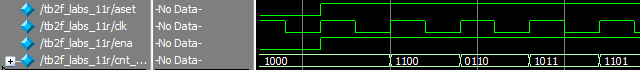
\includegraphics[width=0.9\textwidth]{test3r_results}
		\vspace{0.1cm}
	\end{subfigure}
	\begin{subfigure}{\textwidth}
		\centering
		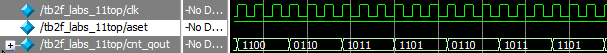
\includegraphics[width=0.85\textwidth]{test3top_results}
	\end{subfigure}
	\caption{Результаты тестов второго класса с чтением файлов}
	\label{fig:test3_results}
\end{figure}

В листинге \ref{code:test3_error} приведен вывод результатов теста верхнего уровня в консоль при внесении ошибок в ожидаемые значения.
\begin{lstlisting}[caption=Результаты ошибочного теста второго класса с чтением файлов, label=code:test3_error, style=console]
run -all
# Expected  6, got  8
# Expected 11, got 12
# Expected 13, got  6
# Expected  6, got 11
#    Time: 1080 ns  Iteration: 1  Instance: /tb2f_labs_11top
\end{lstlisting}

\section{Выводы}

В ходе лабораторной работы на языке Verilog описаны тесты первого и второго классов для каждого из модулей исследуемого устройства и для описания верхнего уровня. Тестирование разработанного устройства показало, что результаты совпадают с ожидаемыми и устройство работает верно.

\end{document}